%% amssamp1.tex is nearly identical to amssamp2.tex, except
%% that amssamp2.tex uses the [twocol] option to produce
%% two-column text.

%\documentclass{ametsoc}

\documentclass[twocol]{ametsoc}

%%%%%%%%%%%%%%%%%%%%%%%%%%%%%%%%
%%% To be entered only if twocol option is used

\journal{jtech}
\usepackage{graphicx}
\usepackage{caption}
\usepackage{subcaption}
\usepackage{hyperref}
\usepackage{url}
%  Please choose a journal abbreviation to use above from the following list:
% 
%   jamc     (Journal of Applied Meteorology and Climatology)
%   jtech     (Journal of Atmospheric and Oceanic Technology)
%   jhm      (Journal of Hydrometeorology)
%   jpo     (Journal of Physical Oceanography)
%   jas      (Journal of Atmospheric Sciences)	
%   jcli      (Journal of Climate)
%   mwr      (Monthly Weather Review)
%   wcas      (Weather, Climate, and Society)
%   waf       (Weather and Forecasting)
%   bams (Bulletin of the American Meteorological Society)
%   ei    (Earth Interactions)

%%%%%%%%%%%%%%%%%%%%%%%%%%%%%%%%
%Citations should be of the form ``author year''  not ``author, year''
\bibpunct{(}{)}{;}{a}{}{,}

%%%%%%%%%%%%%%%%%%%%%%%%%%%%%%%%

\title{A ten year radar climatology of rainfall over Portland, Maine.}

\authors{Scott Collis\correspondingauthor{Scott Collis, Argonne National Laboratory, 
Environmental Science division, 
9700 South Cass Ave, Argonne, IL 60514} }

\affiliation{Environmental Science Division, Argonne National Laboratory} 

\email{scollis@anl.gov}

%\extraauthor{Extra Author}
%\extraaffil{Affiliation, City, State/Province, Country}



\abstract{This paper describes a Department of Homeland Security, Regional Resiliency Assessment 
Program study into precipitation over Portland, Maine carried out by Argonne National Laboratory. The
 primary data source is scanning weather radar which collects information about precipitating particles
  over a large (250km plus) domain. The Python ARM radar Toolkit was used to retrieve rainfall rates 
  from the local radar (in the Gray township outside of Portland) and map them onto a 250m resolution
   grid over a 100km domain. Using Argonne's large scale cluster, Blues, the problem was mapped to 
   10 years worth of data, just over 600,000 ten minute volumes or just over 10TB of data. Each time 
   step was reduced to two numbers: The domain mean and maximum rainfall rate to allow easy 
   indexing of the data set. In addition the diurnal (daily) cycle of precipitation was studied as was the seasonal cycle. }

\begin{document}
\maketitle


\section{Introduction}
\label{sec:intro}
Quoting directly from the Department of Homeland Security's (DHS) webpage : \textit{The 
Regional Resiliency Assessment Program (RRAP) is a cooperative assessment of specific
 critical infrastructure within a designated geographic area and a regional analysis of the
surrounding infrastructure. The RRAP is led by the Department of Homeland Security
and addresses a range of hazards that could have regionally and nationally significant
 consequences. Each year, the Department selects these voluntary and non-regulatory 
RRAP projects with input and guidance from federal and state partners.} Argonne is a
partner in the RRAP project over Portland, Maine. One specific aspect we are looking
at in critical drainage infrastructure and what will be required in a changing climate
scenario. Dynamical downscaling (eg \cite{wang}) where a high resolution computer
 model is used to simulate what happens within the 100km climate model grid cell, 
 is coming into more common usage. However, the key science question being asked by
  Argonne researchers is: Is the 12km resolution of these models enough to resolve high intensity  
localized precipitation events?

To this end our team carried out a study that involves using NOAA weather radars, known as 
Weather Surveillance Radars -1988 Doppler or WSR-88D (\cite{crum_wsr-88d_1993}) to create high 
resolution rain maps for ingest into hydrological models. These rain maps are then de-resolved or made 
coarser and the impact on stream and culvert flow analyzed over the Portland area. This report only 
deals with the generation of the rain maps and is broken into four sections: This introduction, Background 
information on the tools used and an introduction to radar meteorology, a discussion of the results obtained 
and some thoughts as to future work.  

 
\section{Background}
Data from the WSR-88D radars are freely available both realtime, archived by the National Centers for 
Environmental Information and also, recently in the Amazon Cloud. In order to help the reader understand
the processing that was performed on the radar data to extract geophysical insight we will first give some
basic background in radar meteorology. 

\subsection{NOAA weather radars}
\label{ssec:nexrad}
The National Weather Service operates a network of 160 radars for the monitoring of atmospheric phenomena. 
These transmit pluses of radiation and monitor the reflections, or backscatter, of objects in the pulse's path. The
 radar receives these reflected signals and calculates profiles of data along the path of propagation of the pulse. 
 If the radar stayed still users will receive just one "soda straw" view through the target of study (eg a rainstorm) 
 so, in order to map a volume of space the radar is scanned in azimuth (from north) and elevation (from the horizon).
 This is illustrated in part in fig \ref{fig:radar}. 
\begin{figure}[h]
    \centering
    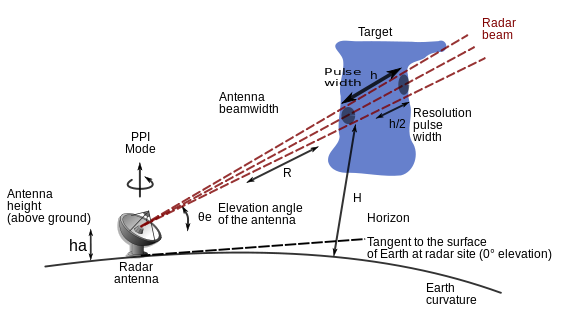
\includegraphics[width=0.95\columnwidth]{radar_prop.png}
    \caption{Cartoon of the propagation of the radar beam through a storm, By Vigneron et Pierre cb - Own work, 
    CC BY-SA 3.0, \href{https://commons.wikimedia.org/w/index.php?curid=4177376}{Link to Wikimedia}}
    \label{fig:radar}
\end{figure}

A single sweep through 360 degrees of azimuth is carried out before the elevation angle is changed. This is called a 
Plan Position Indicator scan or PPI (a historical hangover from when radar images were viewed on cathode ray tube 
displays). One primary measurement radars collect is how effectively the media (eg raindrops) reflects radiation back
 and is called Reflectivity Factor often denoted $\mathrm{Z_e}$. We will skip the derivation and description of this 
 quantity, interested readers are directed to \cite{doviak1984doppler} for more information. An example of a PPI of reflectivity factor is 
 shown in fig \ref{fig:z}. 

\begin{figure}[h]
    \centering
    \begin{subfigure}[b]{0.4\columnwidth}
        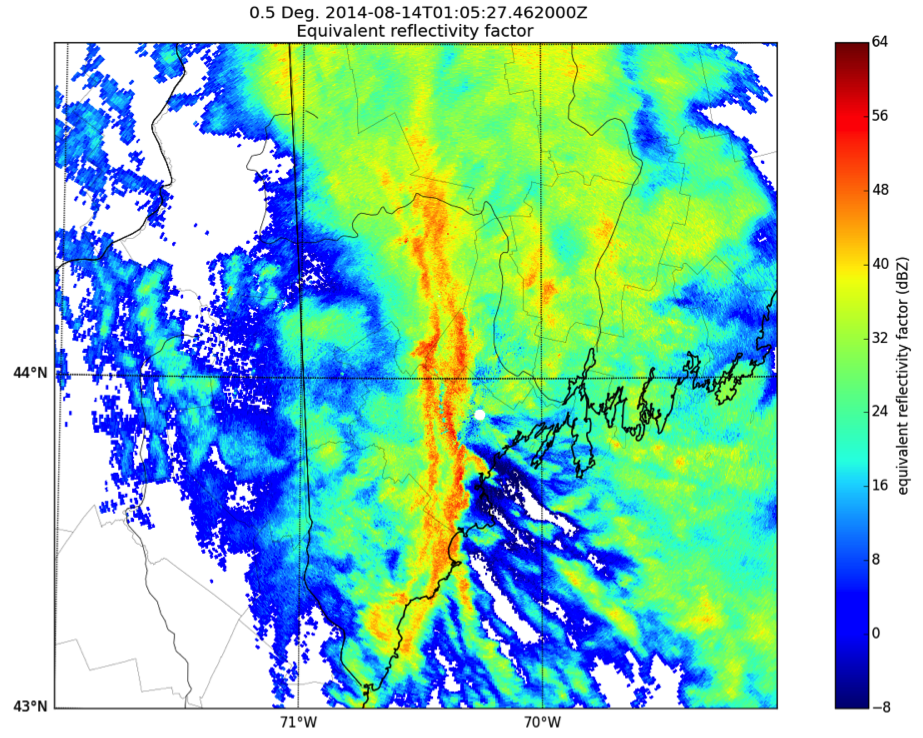
\includegraphics[width=\columnwidth]{refl.png}
        \caption{Radar Reflectivity.}
        \label{fig:z}
    \end{subfigure}
     %add desired spacing between images, e. g. ~, \quad, \qquad, \hfill etc. 
      %(or a blank line to force the subfigure onto a new line)
    \begin{subfigure}[b]{0.4\columnwidth}
        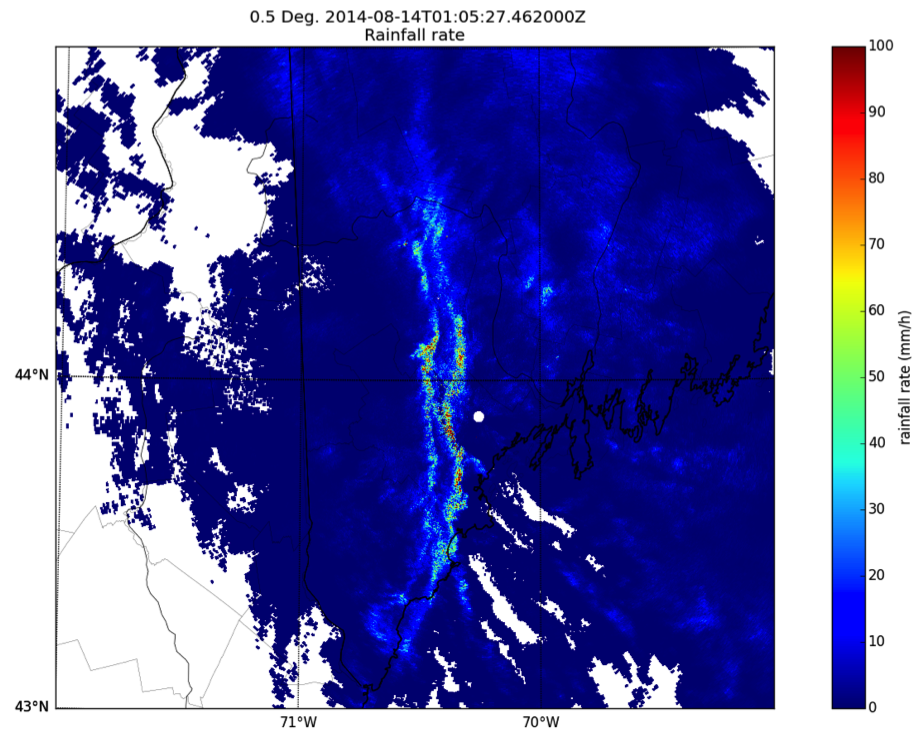
\includegraphics[width=\columnwidth]{rainfall.png}
        \caption{Rainfall rate.}
        \label{fig:rainfall}
    \end{subfigure}
    \caption{Data in the radars native coordinate system of azimuth and range from the lowest elevation sweep of 0.5$^\circ$. }
\end{figure}

If we assume that the volume of the radar pulse contains a number of rain droplets of varying diameter (D) and can be described 
as obeying a number distribution $\mathrm{N(D)}$ (so for a particular Diameter you get a density of rain drops in $\mathrm{m^{-3}}$ 
of N). The reflectivity of raindrops ends up being:
\begin{align*}
Z_e = \int{N(D)D^6dD}
\end{align*}
or the 6$\mathrm{^{th}}$ moment of the drop size distribution. This means a small number of larger drops has a bigger
 impact than increasing the density of smaller drops. 
 
 There have been many papers written on the best way to derive rainfall rates from reflectivity factor and other radar variables. 
 For the purposes of this study where we are more interested in the comparative nature of rainfall patterns we stuck to a simple 
 parametric fit as presented in \cite{gu_polarimetric_2011} of
\begin{equation}
\label{eq:zr}
 Z_e=300R^{1.4}.
 \end{equation}
Equation is inverted to give rainfall rate and an example of this is shown in fig \ref{fig:rainfall}.

\subsection{Application Chain}
\label{sec:ac}
The Python-ARM Radar Toolkit (Py-ART, \cite{heistermann_emergence_2014})  is the main
tool used to perform the steps of: Reading, retrieving rainfall rate, gridding to a 
cartesian grid and writing to a Community standard file format. 
Py-ART is a community data-model drive architecture for interactive development
 of custom processing chains implemented in the Python programming 
language and makes heavy use of the Scientific Python ecosystem (\cite{scipy}). 
Py-ART is community based open source software welcoming
 public contributions on \href{https://github.com/ARM-DOE/pyart}{GitHub}.

Py-ART has a native reader for multiple WSR-88D file formats. The data is read 
into the Py-ART common data model. Rainfall rate in native (antenna) coordinates
of range from the radar, azimuth from north and elevation above the horizon is
 calculated. Then, in order to facilitate easy analysis, the rainfall (in addition to other values) 
is mapped to a regular Cartesian grid with coordinates of meridional and zonal 
(east/west, north/south) displacement from the radar location. Mapping is 
achieved using an inverse distance weighted objective analysis system. Each grid point in the
 destination grid is assigned a radius of influence. Radar gates falling within that radius are 
 averaged to that point using a exponential inverse distance weighting (after \cite{barnes_technique_1964}).
  Py-ART calculates the optimal variable radius of influence. 

Since the radar samples azimuthally the resolution, $R$, of the data 
varies as a function of distance given by

\begin{equation}
R = 2d\tan(\frac{1}{2}\theta_{fwhm})
\end{equation}

where $\theta_{fwhm}$ is the radar beam width and $d$ is the distance of the range gate from the radar. 
The WSR-88D radars have a beam width of 1 degree so at a distance of 30km the resolution will be approximately
 500m. Given we wish to oversample near the city of Portland which is approximately 20km from the radar we chose
 a grid spacing of 200m resulting in a grid with 501 by 501 elements and a domain of 100km. 

 \begin{figure}[h]
    \centering
    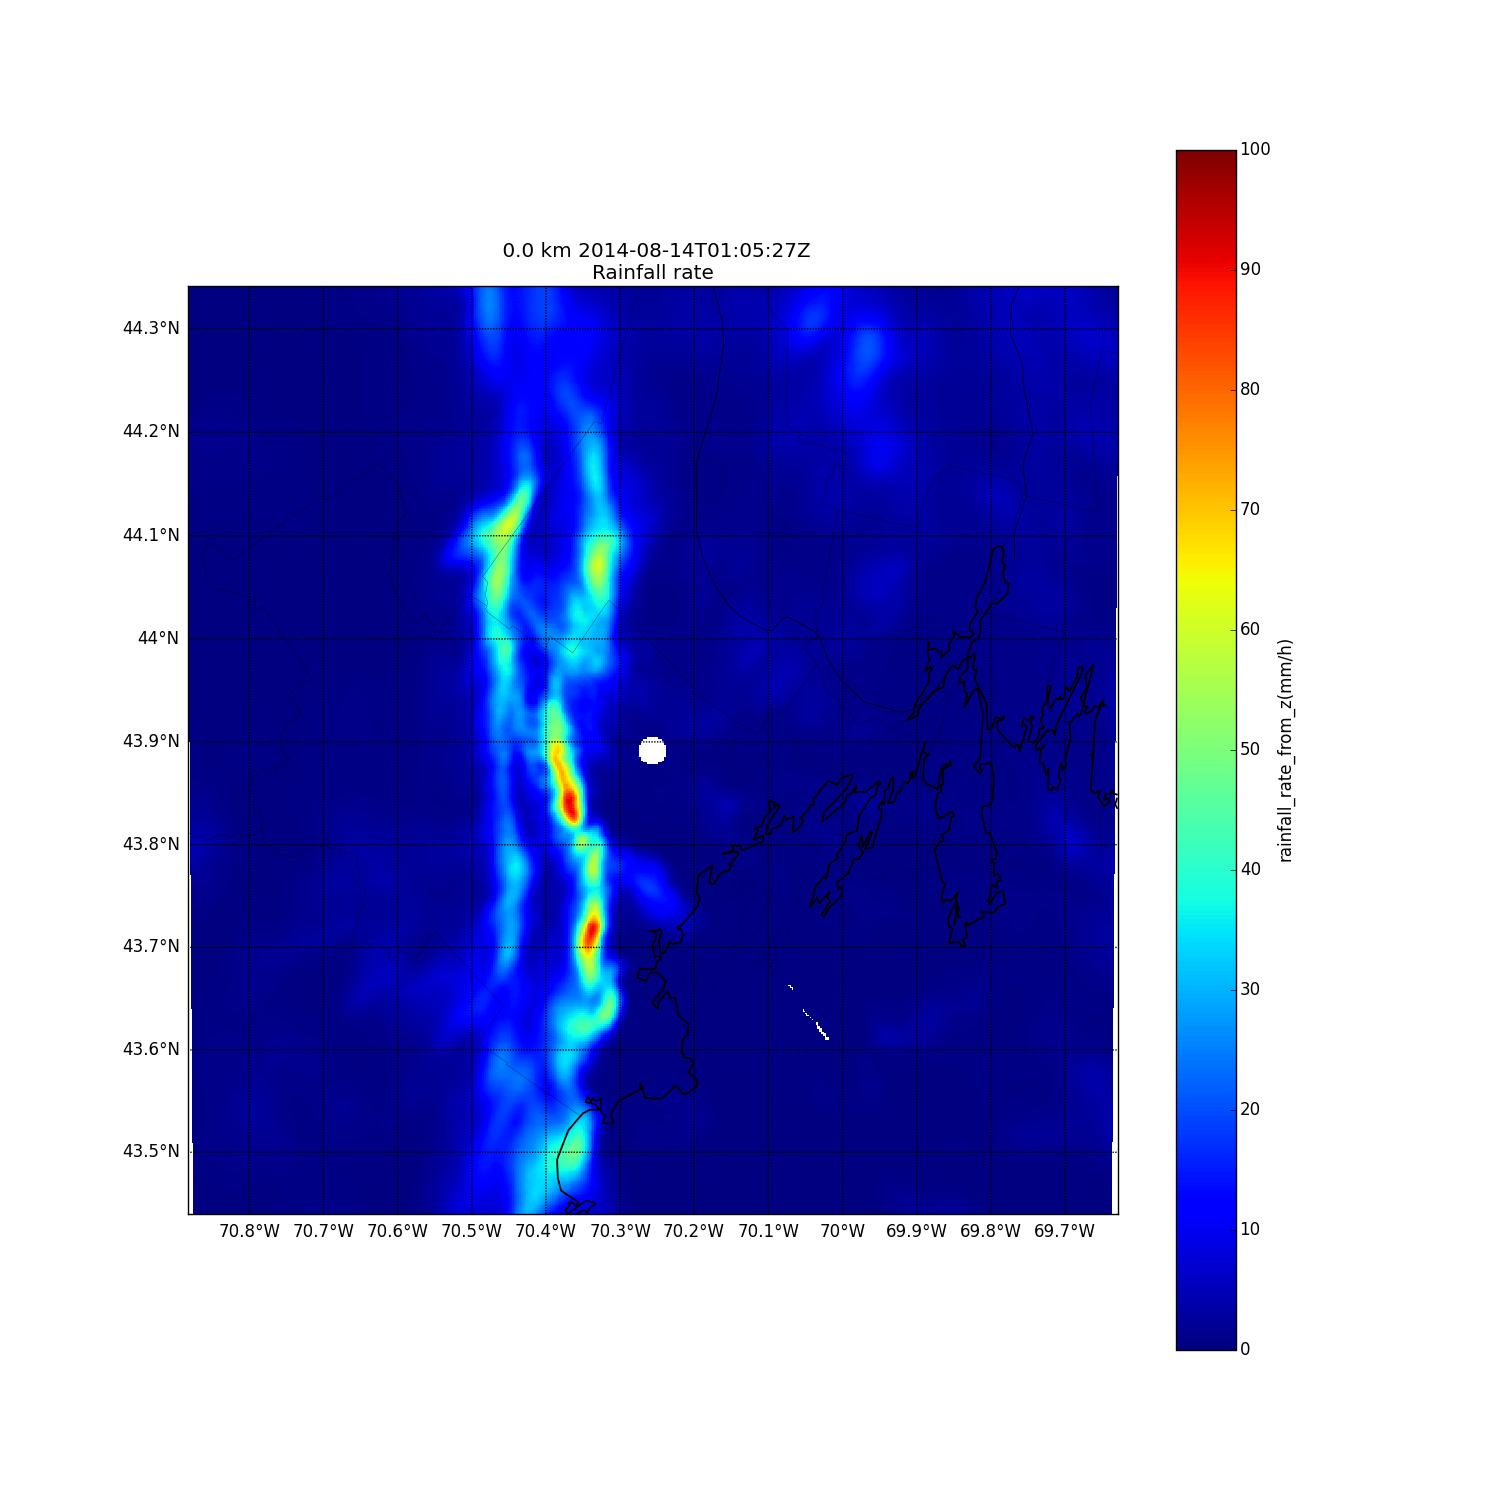
\includegraphics[width=0.95\columnwidth]{mapped.png}
    \caption{Rainfall rates as shown in fig \ref{fig:rainfall} mapped to a Cartesian grid around the Portland, Maine area.}
    \label{fig:mapped}
\end{figure}

Figure \ref{fig:mapped} shows a mapping of rainfall rates calculated in fig \ref{fig:rainfall}. This data is then saved to a NetCDF file that complies 
with the Climate Forecasting conventions (see http://cfconventions.org/).


\subsection{Data Informatics}
Section \ref{sec:ac} gave an overview of the application chain for one volume. Given that our data set consists of hundreds of thousands of files 
we need an effective way to reduce the problem and map to a large scale cluster. Fortunately, due to the granularity (one granule = one file = one volume) 
the problem is \textit{pleasantly} parallel. Also fortunately the Scientific Python ecosystem has recently been enhanced by project Jupyter (\cite{jupyter})
which includes methods for simply mapping a serialized problem to a list of parameters (eg a file list) as shown in fig \ref{fig:cluster}. 
\begin{figure}[h]
    \centering
    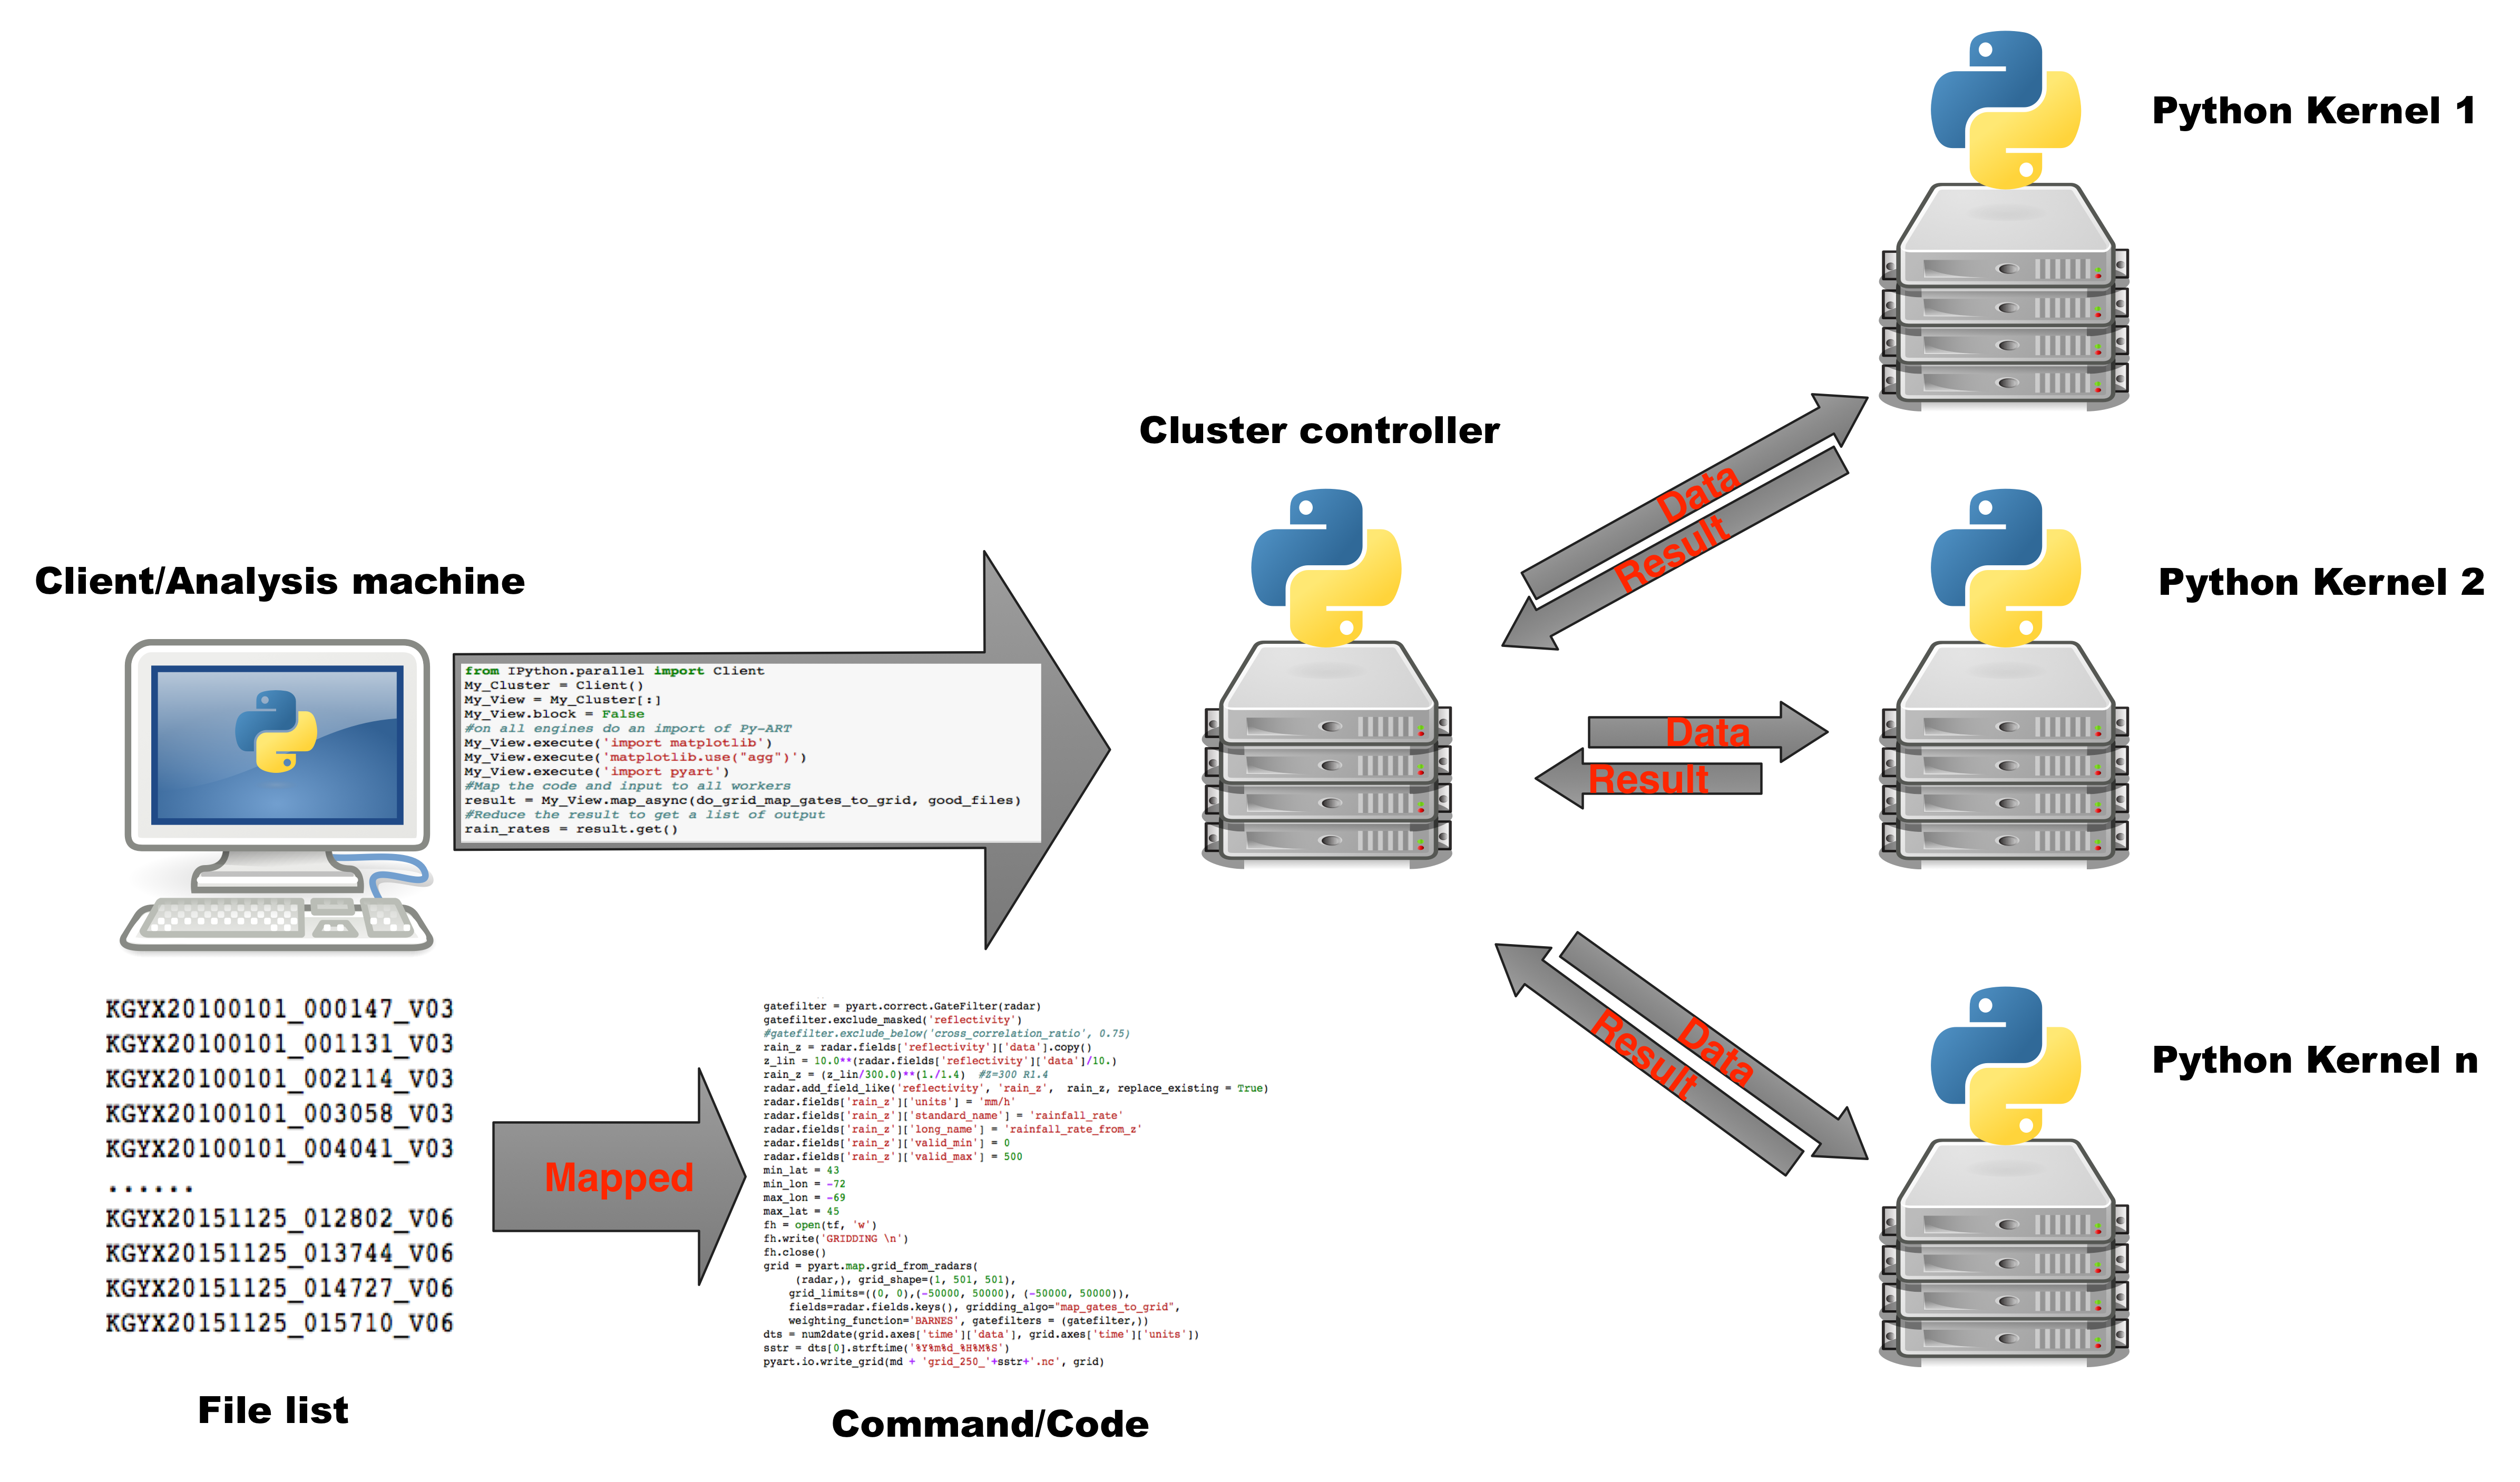
\includegraphics[width=0.95\columnwidth]{cluster.png}
    \caption{pictorial representation of a Jupyter cluster being used for Map-Reduce.  }
    \label{fig:cluster}
\end{figure}

Files containing data from the Portland WSR-88D (Code: KGYX) were staged to Argonne's Blues cluster with 310 compute nodes, 
64 GB of memory on each node, 16 cores per compute node (Intel Sandy Bridge) 4,960 compute cores available and a theoretical
 peak performance of 107.8 TFlops. Mapping the 670,353 files that made up the study was performed using several jobs ranging from
 64 to 1024 cores taking a wall time of just over 48 hours. Each job produced three output files: a NetCDF file containing the gridded data,
 plots such as those shown in fig \ref{fig:mapped} and a simple ascii file with the mean of the rainfall values in the domain and the 
 maximum value in the domain.
 


\section{Results}
Once execution was complete the rainfall grids were archived and the domain mean values were moved off the cluster for analysis (the 
advantage of reducing several Tb down to ~100Mb). Figure \ref{fig:clim} shows the domain mean rainfall rate (for the domain shown 
in fig \ref{fig:rainfall}) as a function of time. Since the temporal resolution is of the order of 10 minutes the figure does not have the resolution
to show individual events. 
\subsection{Rainfall look up table}
\begin{figure}[h]
    \centering
    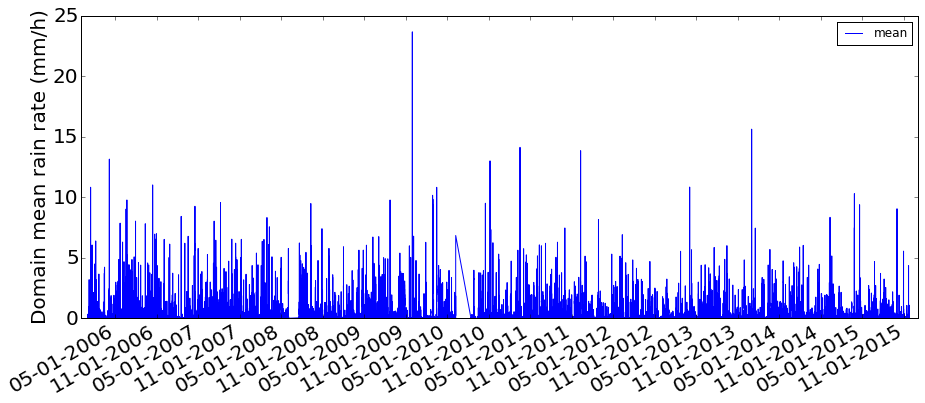
\includegraphics[width=0.9\columnwidth]{climatology.png}
    \caption{Domain mean rainfall rate as derived from a reflectivity/rainfall relationship using the KGYX WSR-88D radar. }
    \label{fig:clim}
\end{figure}
For the purposes of RRAP and understanding rainfall over Portland the rainfall rates can act as a look up table to identify
rainfall events for further study. While domain mean rainfall rate is a crude metric all the grid are archived allowing quick 
reanalysis. Due to noise in the radar signal and scattering off objects like buildings (called clutter) the minimum signal 
is 0.05 mm/hr so anything less than this is considered "no rain". 

\subsection{Brief Analysis of Rainfall Variability}
We can look at the temporal distribution of rainfall by partitioning it into hourly and monthly percentiles and means. 
\begin{figure}
    \centering
    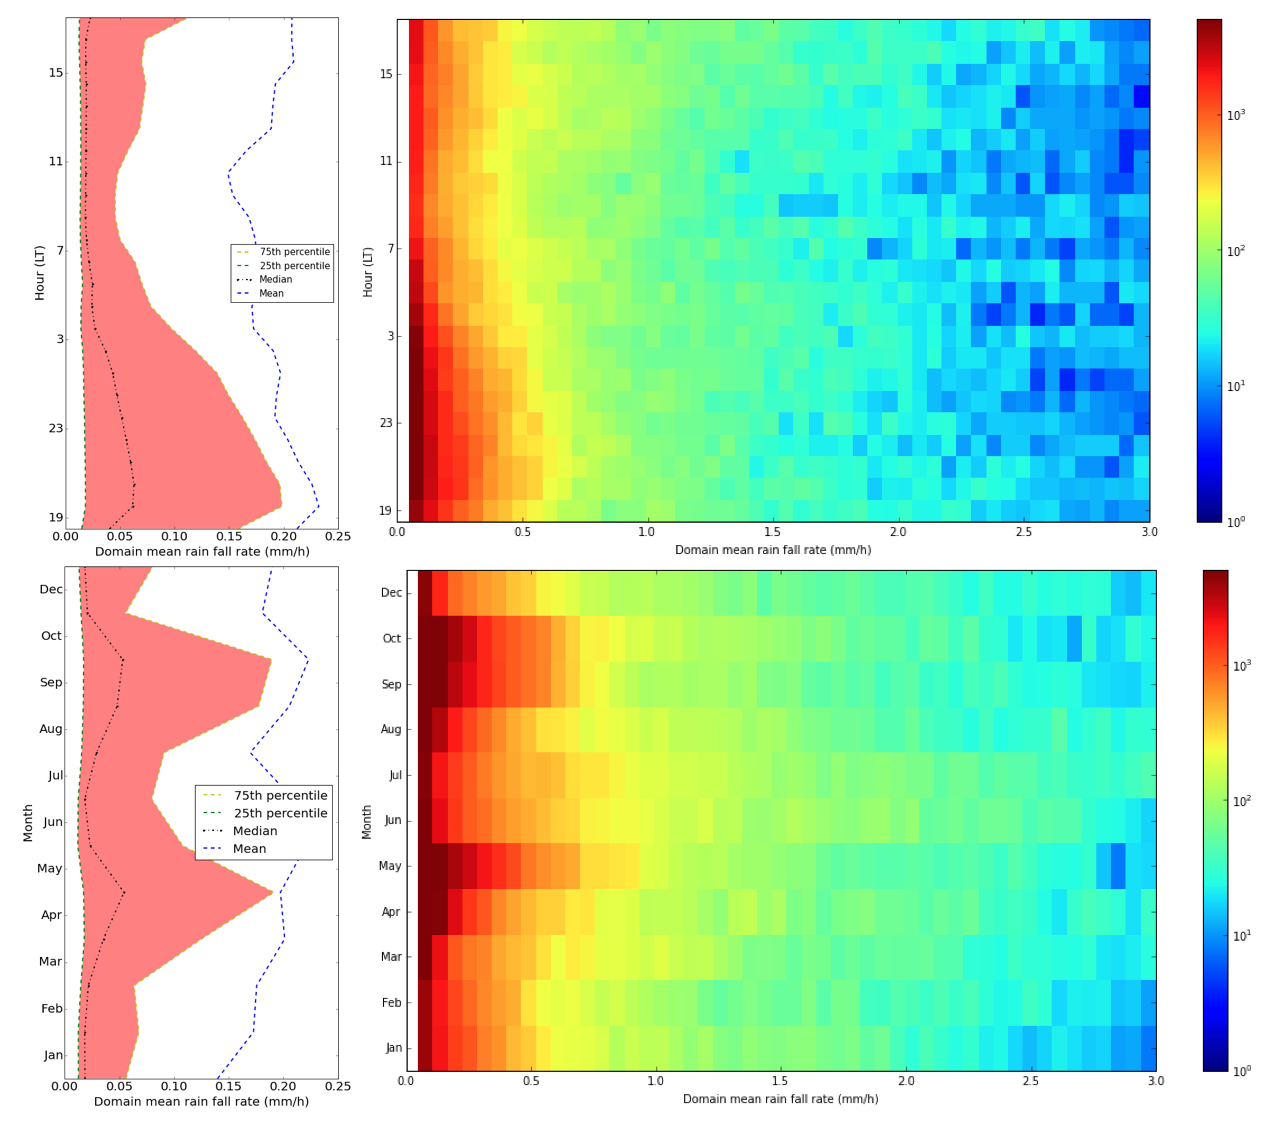
\includegraphics[width=1.0\columnwidth]{var.png}
    \caption{Rainfall statistics broken down into hourly and monthly distributions.  Then left hand side shows percentiles of 
    rainfall events and the mean.  The right hand side shows, for each hour or month, a histogram of rainfall events using a 
    colormap. Red colors show high counts blue shows rare events.}
    \label{fig:var}
\end{figure}
Rainfall rates are spilt into separate distributions based on the hour of the day (local time) and the month of the year. 
Based on these distributions the 25th, median and 75th percentiles of rainfall rate are calculated. These are show in 
the lefthand panels of fig \ref{fig:var}. In addition, histograms of the rainfall rate for each hour and month are calculated 
and is shown in the right hand panels. These histograms are stacked in time, so all the rainfall rates for a month (say, March) 
are grouped and then the rates are sorted into bins. The first bin is 0.1 to 0.2 mm/h so there will be a certain number of times 
we observe that rain rate, in the month of March, in our study, it was ~1000 samples giving it the red color in fig \ref{fig:var}. 
A sample is a single radar measurement which occurs approximately every 10 minutes. Very high rainfall values happen 
less frequently. For example, domain mean rainfall rates of 2.9 to 3.0 mm/h in the month of March only occurs 10 times
(note the color scale in fig \ref{fig:var} us logarithmic). Individual histograms for 10-11pm and for the month of October are shown in 
fig \ref{fig:hists}.
Figure \ref{fig:var} highlights many interesting pattens in Portland rainfall. First, given the mean is much greater than the 
median we can see that the rainfall distribution is skewed. That is, a greater contribution towards total rainfall comes 
from the more extreme events than the weaker events. 
The figure also shows a clear diurnal (or daily) cycle with an overnight maximum. This is consistent with many studies 
of rainfall across the globe (eg \cite{nesbitt_diurnal_2003}). This is due to the most widespread systems being more 
intense at night, the physical mechanisms are beyond the scope of this report but it is pleasing to see an expected 
natural and physically consistent variation apparent in the data. 
The monthly data shows a clear seasonal cycle with the percentiles exhibiting a fall and spring peak. However inspection
 of the mean and histograms to the right shows that while mid-scale events are more populous in spring and fall higher end 
 events occur in summer as well. 
 
 \begin{figure}
    \centering
    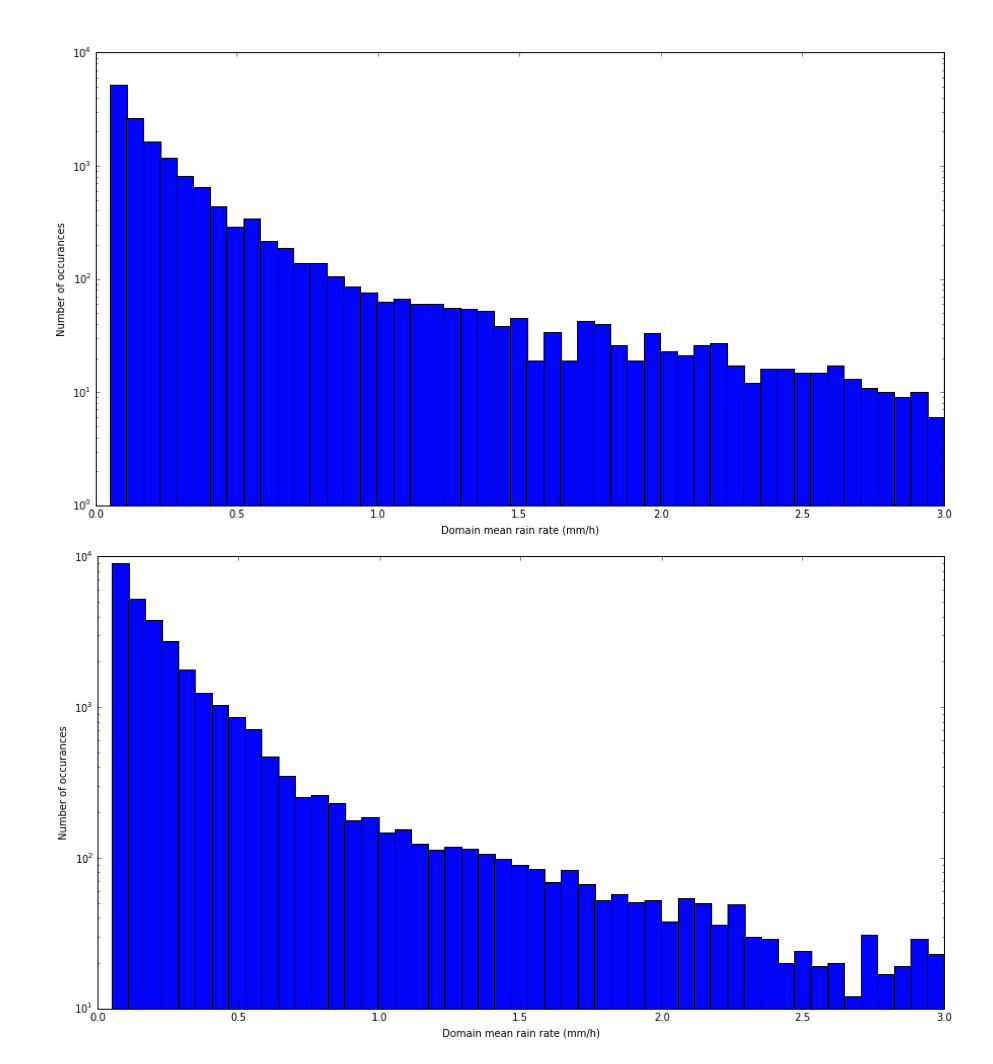
\includegraphics[width=0.8\columnwidth]{hists.png}
    \caption{Histograms of domain mean rainfall rates for 10pm to 11pm at night (top) and the month of October (bottom). }
    \label{fig:hists}
\end{figure}
 
 So far the scope of our work has been limited to investigating bulk statistics. In order to look at trends and to comment on if 
 heavy precipitation events are increasing would entail more rigorous data quality work to ensure technical issues do not lead 
 to erroneous findings. 

\section{Conclusions and Future Work}
Ten years of radar data from Portland, Maine, were used to construct a decade's worth or rainfall rate grids. These grids have 
been handed over to the hydrology group at Argonne and will be used to investigate the scale dependance of rainfall. For each 
grid the domain mean rainfall was calculated both as a health and status monitor and as a look up table to quickly find events of 
interest to the team. This data turned out to be interesting in its own right. The rainfall record shows interesting daily and monthly 
cycles with an overnight maximum  and spring and fall peaks. The rainfall record is also highly skewed with the median rainfall rate
being much less than the mean. This indicates that Maine gets much of its rainfall from heavier events. 

This rainfall retrieval technique outlined in sec \ref{ssec:nexrad} was crude as the initial aim of the study was purely to create grids 
for use in the hydrological modeling.  In the future we wish to improve the quality control of the data to filter out various phenomena 
that corrupt the data and to also detect the presence of snow and treat it differently to rain. The retrieval and cluster framework is 
already set up (see \href{https://github.com/scollis/high_resolution_hydrology}{this link to the GitHub repository})
 so improvements can be made and rerunning the climatology is only a matter of core hours.
 
There are two main areas for future work beyond quality control improvements: Comparison with regional downscaling hindcasts and 
the development of more sophisticated metrics than just domain mean. 

Signatures apparent in fig \ref{fig:var} should also be present in rainfall produced by regionally downscaled climate models. We are already 
working with scientists here at Argonne comparing our radar measurements to that produced by forcing high resolution models with the 
CMIP5 climate models. The period of overlap is from 1995 to 2005. NEXRAD is only reliable after 1995 (getting considerably better in 2001 in 
terms of uptime) and CMIP5 only goes to 2005. We are performing this study both over Portland and Oklahoma where the DoE Atmospheric 
Radiation Measurement Research program has extensive instrumentation \cite{ackerman_atmospheric_2003}. These studies become more 
important as the climate modeling community gears up for CMIP6, where we will have a much greater overlap between the hindcast and radar
 data. Radar climatologies like those presented in this report will be key for testing the veracity of various downscaling methodologies. 

As previously mentioned we limited our investigations to looking at bulk means and monthly and daily cycles of precipitation. More detailed investigations
 into the quality of the data and the application of very careful statistical analysis may allow trends to be investigated, including comparisons with the 
 National Climate Assessment (\cite{climchange}), specifically with figure 2.18. 
 
As mentioned previously in this report domain mean rainfall is a simple but not sufficient way to index the contents of the rainfall grids. We wish 
to extend this study to identify "fingerprints of severity" in the rainfall grids. An example would be the area of the grid over a certain rainfall rate 
threshold. We then wish to collect information from atmospheric reanalyses (such as atmospheric instability indexes) to do an ingredients based 
study into what causes extreme rainfall in Maine. We can then look at climate models and see if these ingredients will be more or less likely in 
future climate scenarios thus enabling us to make data driven comments on the likelihood of extreme rainfall in the Portland area going forward. 



%%%%%%%%%%%%%%%%%
%ACKNOWLEDGMENTS
%%%%%%%%%%%%%%%%%

\acknowledgments{}
This report has been created by UChicago Argonne, LLC, Operator of Argonne National Laboratory ("Argonne"). 
Argonne, a U.S. Department of Energy Office of Science laboratory, is operated under Contract No. DE-AC02-06CH11357. 
This research was supported by the Office of Biological and Environmental Research of the U.S. Department of Energy as
 part of the Atmospheric Radiation Measurement Climate Research Facility and the Department of Homeland Security
 Regional Resiliency Assessment Program. We gratefully acknowledge the computing resources provided on Blues,
 a high-performance computing cluster operated by the Laboratory Computing Resource Center at Argonne National Laboratory.
 
 We wish to thank Duane Verner, Thomas Wall and Eugene Yan for useful discussions during this work and Jonathan Helmus for his tireless support 
 of Py-ART. We also wish to thank all the contributors to Py-ART and the Scientific Python Ecosystem. 
%%%%%%%%%%%%%%%%%
%APPENDIXES
%%%%%%%%%%%%%%%%%
%\appendix
%\appendixtitle{Appendix Title}
%
%\subsection*{Appendix section head}
%
%Here is a sample appendix.
%\begin{equation}
%\frac{
%pf \cos\phi}
%{p^0|\nabla h\bar q|(d\theta_0/dz)}
%\end{equation}
%
%\appendix[B]
%\appendixtitle{Second Appendix Title}
%\subsection{Sample appendix section head}
%Second appendix example.
%\subsection{Sample appendix section head}
%\begin{equation}
%\left(\frac{\partial\bar q}{\partial x}
%\overline{U'\theta'} +
%\frac{\partial\bar q}{\partial y}
%\overline{V'\theta'}\right) 
%\end{equation}


%%%%%%%%%%%%%%%%%
%REFERENCES
%%%%%%%%%%%%%%%%%

\bibliographystyle{ametsoc2014}
\bibliography{zotero}

%%%%%%%%%%%%%%%%%
% TABLES
%%%%%%%%%%%%%%%%%

%\begin{table}
%\caption{Percentage of variance explained by the first four
%EOFs for the North Pacific Bx. The degree of separation between
%EOF1 and EOF2 and EOF2 and EOF3, based on the North et al.
%(1982) criterion, is indicated by good (GD) and not good or marginal
%(NG).}
%\begin{tabular*}{\hsize}{@{\extracolsep\fill}lcccccc@{}}
%\topline
%Month& EOF1& Split &EOF2& Split& EOF3& EOF4\\
%\midline
%\ Jan& 29& NG& 24& GD& 10& 5\\
%\ Feb& 39& GD& 20& GD& \phantom{1}7 &6\\
%\ Mar& 31& GD& 14& NG& 10& 6\\
%\ Apr& 23& GD& 14& NG& 10& 7\\
%\ May& 19& GD& 12& NG& 10& 7\\
%\ Jun& 19& GD& 12& NG& 10& 9\\
%\ Jul& 18& NG &13& NG& \phantom{1}9& 7\\
%\ Aug& 18& NG& 13& NG& 11& 9\\
%\ Sep &17& NG& 13& NG& 10& 8\\
%\ Oct &16& NG& 13& GD& \phantom{1}8& 7\\
%\ Nov &19 &NG& 16& NG& 11& 8\\
%\ Dec& 33& GD& 18& GD& 10& 6\\
%\botline
%\end{tabular*}
%\end{table}

%
%
%\begin{table}
%\centering
%\caption{Years selected for anomaly composites for the positive
%phase of $B^x$ EOF1.}
%\begin{tabular}{lc}
%\topline
%Month& Yr of positive phase\\
%\midline
%\ \ Jan& 1961, 1969, 1978, 1979, 1988, 1990, 1992, 1994\\
%\ \ Feb& 1964, 1977, 1978, 1980, 1983, 1986, 1988, 2000, 2001\\
%\ \ Mar& 1970, 1973, 1979, 1980, 1984, 1988, 2000\\
%\ \ Apr& 1959, 1961, 1962, 1963, 1968, 1972, 1983, 2002\\
%\ \ May& 1971, 1984, 1993, 1996, 2000\\
%\ \ Jun& 1981, 1983, 1984, 1993, 1998\\
%\ \ Jul& 1961, 1972, 1973, 1978, 1994, 2000\\
%\ \ Aug& 1967, 1970, 1973, 1978, 1994, 1999\\
%\ \ Sep& 1975, 1977, 1988, 1989, 1994, 1998, 1999\\
%\ \ Oct& 1962, 1977, 1998, 1999, 2001\\
%\ \ Nov& 1985, 1986, 1987, 1988, 1991, 1998\\
%\ \ Dec& 1957, 1968, 1972, 1978, 1979, 1990\\
%\botline
%\end{tabular}
%\end{table}
%
%\begin{table}
%\centering
%\caption{Years selected for anomaly composites for the negative
%phase of $B^x$ EOF1.}
%\begin{tabular}{lc}
%\topline
%Month& Yr of negative phase\\
%\midline
%\ \ Jan&1962, 1963, 1968, 1974, 1991, 1996, 1997\\
%\ \ Feb& 1959, 1963, 1971, 1974, 1976, 1979, 1985, 1989, 1990, 1994\\
%\ \ Mar& 1963, 1968, 1972\\
%\ \ Apr& 1984, 1988, 1993, 1996, 1999, 2000\\
%\ \ May& 1961, 1963, 1983, 1987, 1997\\
%\ \ Jun& 1961, 1972, 1978, 1980, 1982, 1986\\
%\ \ Jul& 1964, 1974, 1980, 1983, 1986, 1988, 1993\\
%\ \ Aug& 1980, 1987, 1991, 1993, 1997\\
%\ \ Sep& 1959, 1963, 1969, 1983, 1985, 1993\\
%\ \ Oct& 1957, 1986, 1993, 1996, 1997\\
%\ \ Nov& 1958, 1968, 1970, 1982, 1997\\
%\ \ Dec& 1969, 1974, 1976, 1985, 1998, 1999, 2000, 2001\\
%\botline
%\end{tabular}
%\end{table}

%%%%%%%%%%%%%%%%%
% FIGURES
%%%%%%%%%%%%%%%%%

%\begin{figure}[t]
%\centerline{\includegraphics[width=\textwidth]{figone.pdf}}
%
%\caption{Climatology of $Bx (10^{-6} s^{-1}$, color) and $U^{200}$(m s$^-1$,
%contours) for (a) February and (b) August; $\overline{V'\theta'}^{850}$
%(K m s$^-1$, color) and 
%$\overline{V'V'}^{200}$
%(m$^2$ s$^{-1}$, contours) for (c) February and (d) August; MR$^{z850}$ 
%(10$^{-3}$ m$^2$ s$-2$, color) and $U^{1000}$ (m s$^{-1}$, contours) 
%for (e) February and (f) August;
%and SST (K, color) and $F_h$ [10$^5$ J m$^{-2}$ (6 h)$^{-1}$] for (g)
%February and (h) August. Red rectangles indicate the domain of EOF
%calculations.} \label{fig1} 
%\end{figure}
%
%\begin{figure}[p]
%\centerline{\includegraphics{FigTwo.pdf}}
%\caption{As in Fig.~10, but for (a),(b) September EOF1; (c),(d) September EOF2; (e),(f) October EOF1; (g),(h) October EOF2; and
%(i),(j) December EOF2.}
%\end{figure}
%
%\begin{figure}
% \centerline{\includegraphics[width=19pc]{figure01.pdf}}
%\appendcaption{A1}{Here is an appendix, single column figure caption.}
%\end{figure}
%



\end{document}





